\documentclass[12pt]{article}
\usepackage{background}
\usepackage{graphicx}
\usepackage[margin=1in]{geometry}
\usepackage{setspace}
\usepackage{hyperref}
\usepackage{xcolor}
\usepackage{tikz}
\usepackage{listings}
\usepackage{xcolor}
\usepackage{float}
\usepackage{subcaption}
\usepackage{circuitikz}
\usepackage[justification=centering]{caption}

\lstset{
	language=Python,
	backgroundcolor=\color{black!5},
	basicstyle=\ttfamily\small,
	breaklines=true,
	keywordstyle=\color{blue},
	commentstyle=\color{green},
	stringstyle=\color{red},
	identifierstyle=\color{black},
	morekeywords={def,class},
	morekeywords={import, as},
	frame=single,
	rulecolor=\color{black},
	tabsize=4,
	showstringspaces=false
}

\backgroundsetup{
	scale=0.5,
	color=black,
	opacity=0.1,
	angle=0,
	position=current page.center,
	vshift=-5cm,
	hshift=0cm,
	contents={
\includegraphics[width=\paperwidth, height=\paperheight]{figs/logo.jpg}}
}

\setcounter{secnumdepth}{2} % Enables numbering for sections and subsections
\setcounter{tocdepth}{2} % Includes subsections in the TOC

\title{\textbf{Scientific Calculator}}
\author{J.KEDARANANDA\\EE24BTECH11030}
\date{March 2025}

\begin{document}
	
	\maketitle
	\tableofcontents
	\newpage
	
	% --- Existing Content Starts Here ---
	
	\section{Introduction}
	This project implements a scientific calculator using an Arduino microcontroller with a 5×5 keypad matrix and an LCD display. The calculator is capable of performing both basic arithmetic operations and advanced mathematical functions such as trigonometric calculations, logarithms, and exponentiation.
	
	The scientific calculator serves as a practical application of embedded systems design and programming, combining hardware interfacing with mathematical computation algorithms. As processors become more powerful and interfaces more user-friendly, calculators continue to be essential tools in engineering, science, and education.
	
	\subsection{Project Objectives}
	The main objectives of this project are:
	\begin{itemize}
		\item Develop a functional scientific calculator using the Arduino platform
		\item Implement a user-friendly interface using a 5×5 key matrix and LCD display
		\item Support basic arithmetic operations: addition, subtraction, multiplication, and division
		\item Include advanced mathematical functions: trigonometry, logarithms, and power functions
		\item Create an efficient and responsive system using low-level programming techniques in C
	\end{itemize}
	
	\subsection{Scope of the Project}
	The scientific calculator provides a comprehensive range of functions comparable to a standard scientific calculator, including:
	\begin{itemize}
		\item Basic operations: addition, subtraction, multiplication, division
		\item Power and square root functions
		\item Trigonometric functions: sine, cosine, tangent
		\item Inverse trigonometric functions (with shift key)
		\item Natural and base-10 logarithms
		\item Support for constants like Euler's number (e)
	\end{itemize}
	
	\section{Hardware Components}
	The project utilizes several key hardware components to build a functional calculator system. Each component plays a specific role in the overall design and functionality.
	
	\subsection{Arduino UNO}
	The Arduino UNO serves as the central microcontroller unit of the calculator. Based on the ATmega328P microcontroller, it provides:
	\begin{itemize}
		\item 6 analog inputs
		\item 16 MHz crystal oscillator
		\item USB connection for programming
		\item 32 KB Flash memory for storing program code
		\item 2 KB SRAM for runtime operations
	\end{itemize}
	
	The Arduino's ability to handle both the keypad input scanning and LCD display control simultaneously makes it ideal for this application.
	\begin{figure}[h]
		\centering
		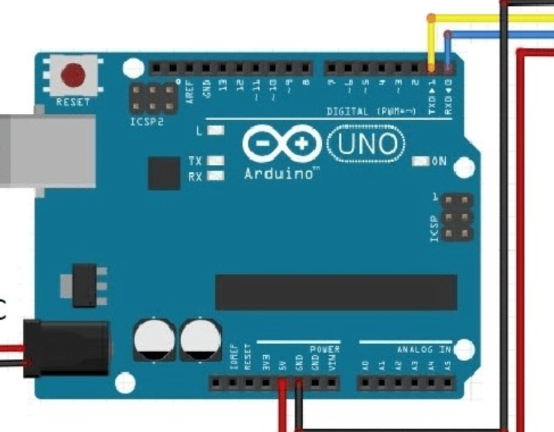
\includegraphics[width=0.4\textwidth]{figs/arduino}
	\end{figure}
	\subsection{16×2 LCD Display}
	The 16×2 LCD (Liquid Crystal Display) module provides the visual interface for the calculator, with:
	\begin{itemize}
		\item 16 characters per line, 2 lines total
		\item HD44780 compatible controller
		\item 4-bit interface mode to minimize pin usage
		\item 5×8 pixel character display
		\item Contrast adjustment capability
		\item Backlight for better visibility
	\end{itemize}
	
	This display size provides sufficient space to show both the input expressions and calculation results while minimizing the project's physical footprint.
	\begin{figure}[h]
		\centering
		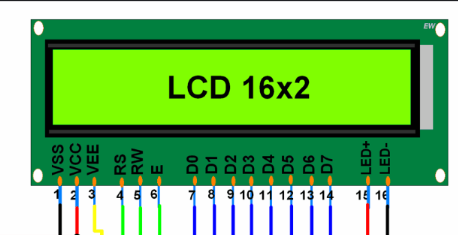
\includegraphics[width=0.4\textwidth]{figs/lcd.png}
	\end{figure}
	\subsection{5×5 Matrix Keypad}
	The custom 5×5 matrix keypad provides the input interface with 25 keys total:
	\begin{itemize}
		\item Numeric keys: 0-9
		\item Basic operation keys: +, -, *, /, =
		\item Advanced function keys: sin, cos, tan, sqrt, log
		\item Special purpose keys: Shift, Clear, decimal point
	\end{itemize}
	
	The matrix arrangement allows for 25 keys while using only 10 I/O pins (5 rows + 5 columns), maximizing input capability with minimal pin usage.
	
	\subsection{Passive Components}
	Additional components used in the circuit include:
	\begin{itemize}
		\item Potentiometer for LCD contrast adjustment
		\item Jumper wires for connections
		\item Breadboard or PCB for mounting
		\item Power supply components
	\end{itemize}
	
	\section{Circuit Connections}
	The calculator circuit integrates the Arduino, LCD display, and keypad matrix through carefully planned connections that maximize I/O efficiency.
	
	\subsection{LCD Connections}
	The 16×2 LCD is connected to the Arduino in 4-bit mode to save I/O pins:
	
	\begin{center}
		\begin{tabular}{|c|c|c|}
			\hline
			\textbf{LCD Pin} & \textbf{Arduino Pin} & \textbf{Function} \\
			\hline
			RS & 13 (PB5) & Register Select \\
			E & 12 (PB4) & Enable \\
			D4 & A2 (PC2) & Data Bit 4 \\
			D5 & A3 (PC3) & Data Bit 5 \\
			D6 & A4 (PC4) & Data Bit 6 \\
			D7 & A5 (PC5) & Data Bit 7 \\
			VSS & GND & Ground \\
			VDD & 5V & Power \\
			V0 & Potentiometer & Contrast Control \\
			\hline
		\end{tabular}
	\end{center}
	
	\subsection{5×5 Keypad Matrix Connections}
	The keypad is arranged in a matrix of 5 rows and 5 columns, requiring 10 I/O pins:
	
	\begin{center}
		\begin{tabular}{|c|c|c|}
			\hline
			\textbf{Keypad Line} & \textbf{Arduino Pin} & \textbf{Configuration} \\
			\hline
			Row 1 & 6 (PD6) & Output (High with Pull-down) \\
			Row 2 & 7 (PD7) & Output (High with Pull-down) \\
			Row 3 & 8 (PB0) & Output (High with Pull-down) \\
			Row 4 & 9 (PB1) & Output (High with Pull-down) \\
			Row 5 & A1 (PC1) & Output (High with Pull-down) \\
			\hline
			Column 1 & 2 (PD2) & Input (Pull-up) \\
			Column 2 & 3 (PD3) & Input (Pull-up) \\
			Column 3 & 4 (PD4) & Input (Pull-up) \\
			Column 4 & 5 (PD5) & Input (Pull-up) \\
			Column 5 & A0 (PC0) & Input (Pull-up) \\
			\hline
		\end{tabular}
	\end{center}
	
	\subsection{Keypad Matrix Layout}
	The 5×5 keypad matrix is organized as follows, with each key mapped to its corresponding character:
	
	\begin{center}
		\begin{tabular}{|c|c|c|c|c|}
			\hline
			\textbf{1} & \textbf{2} & \textbf{3} & \textbf{4} & \textbf{5} \\
			\hline
			\textbf{6} & \textbf{7} & \textbf{8} & \textbf{9} & \textbf{0} \\
			\hline
			\textbf{+} & \textbf{-} & \textbf{*} & \textbf{/} & \textbf{=} \\
			\hline
			\textbf{sin} & \textbf{cos} & \textbf{tan} & \textbf{.} & \textbf{Clear} \\
			\hline
		\end{tabular}
	\end{center}
	
	\subsection{Full Circuit Diagram}
	The complete circuit diagram showing all connections between the Arduino, LCD display, and keypad matrix is shown below:
	
	\begin{figure}[H]
		\centering
		\begin{circuitikz}
			% Arduino representation
			\draw (0,0) rectangle (3,8);
			\node at (1.5,7.5) {Arduino UNO};
			
			% LCD representation
			\draw (7,5) rectangle (12,8);
			\node at (9.5,7.5) {LCD 16x2};
			
			% Keypad representation
			\draw (7,0) rectangle (12,4);
			\node at (9.5,3.5) {5x5 Keypad Matrix};
			
			% LCD connections
			\draw (3,7) -- (7,7) node[midway, above] {RS (PB5)};
			\draw (3,6.5) -- (7,6.5) node[midway, above] {E (PB4)};
			\draw (3,6) -- (7,6) node[midway, above] {D4 (PC2)};
			\draw (3,5.5) -- (7,5.5) node[midway, above] {D5 (PC3)};
			\draw (3,5) -- (7,5) node[midway, above] {D6 (PC4)};
			\draw (3,4.5) -- (7,4.5) node[midway, above] {D7 (PC5)};
			
			% Keypad row connections
			\draw (3,4) -- (7,4) node[midway, above] {R1 (PD6)};
			\draw (3,3.5) -- (7,3.5) node[midway, above] {R2 (PD7)};
			\draw (3,3) -- (7,3) node[midway, above] {R3 (PB0)};
			\draw (3,2.5) -- (7,2.5) node[midway, above] {R4 (PB1)};
			\draw (3,2) -- (7,2) node[midway, above] {R5 (PC1)};
			
			% Keypad column connections
			\draw (3,1.5) -- (7,1.5) node[midway, above] {C1 (PD2)};
			\draw (3,1) -- (7,1) node[midway, above] {C2 (PD3)};
			\draw (3,0.5) -- (7,0.5) node[midway, above] {C3 (PD4)};
			\draw (3,0) -- (7,0) node[midway, above] {C4 (PD5)};
			\draw (3,-0.5) -- (7,-0.5) node[midway, above] {C5 (PC0)};
			
			% Potentiometer for LCD contrast
			\draw (5,8) -- (5,9) -- (7,9) -- (7,8);
			\node at (6,9.3) {Potentiometer};
			\draw (7,7.8) -- (7,9);
		\end{circuitikz}
		\caption{Complete circuit diagram of the scientific calculator}
		\label{fig:circuit-diagram}
	\end{figure}
	
	\begin{figure}[h]
		\centering
		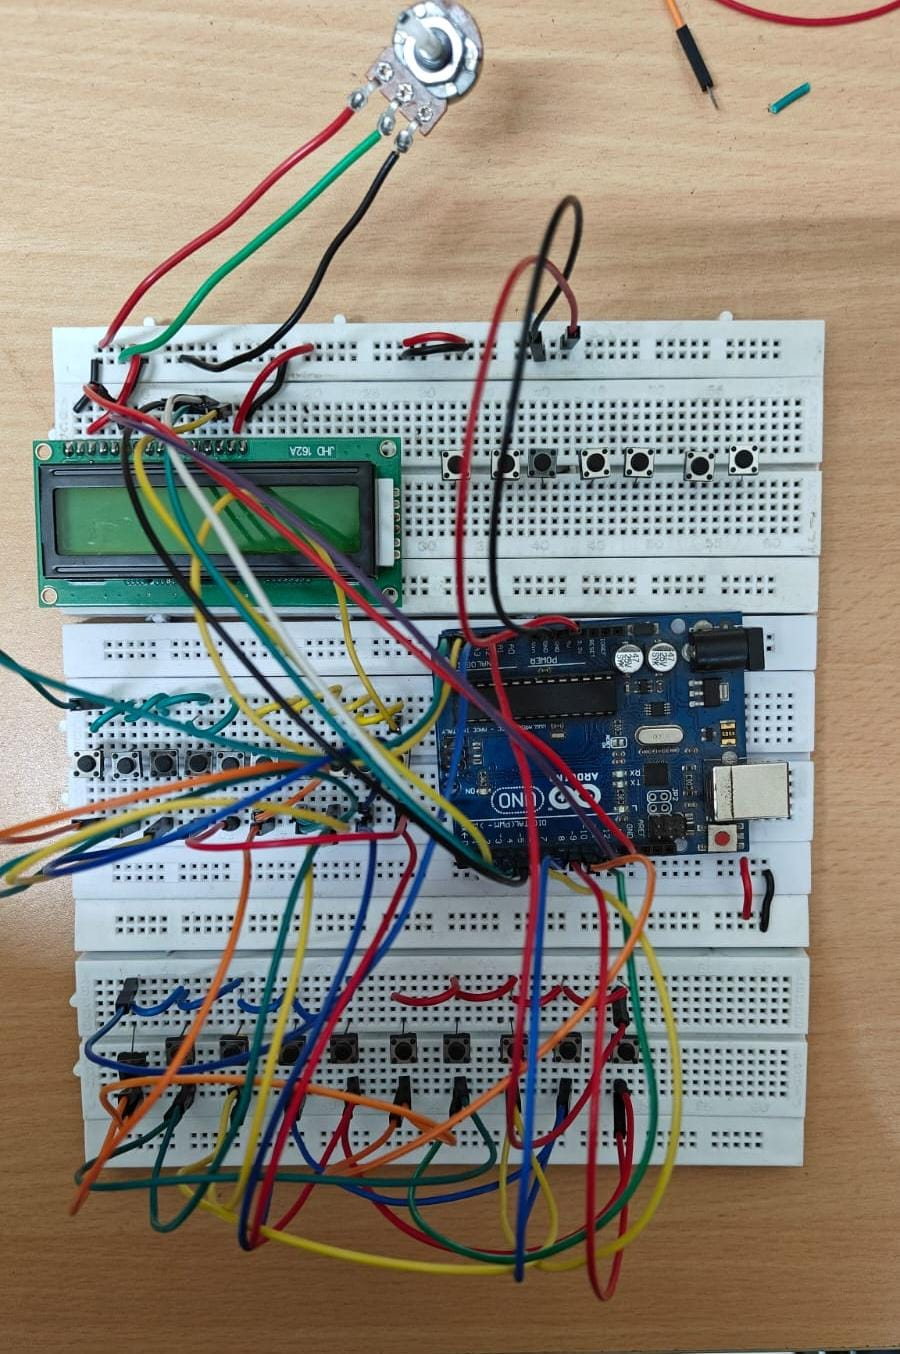
\includegraphics[width=0.4\textwidth]{figs/setup.png}
	\end{figure}
	\section{Hardware Setup}
	The physical assembly of the calculator requires careful attention to detail to ensure proper functionality and reliability.
	
	\subsection{Assembly Process}
	The hardware setup followed these steps:
	
	\begin{enumerate}
		\item Position the 16×2 LCD display and connect the power lines (VDD, VSS)
		\item Connect the LCD control lines (RS, E) to the Arduino
		\item Connect the LCD data lines (D4-D7) to the Arduino
		\item Install the contrast potentiometer and connect it to the LCD's V0 pin
		\item Arrange the 5×5 keypad matrix in a usable configuration
		\item Connect the row pins to the designated Arduino output pins
		\item Connect the column pins to the designated Arduino input pins with pull-up resistors
		\item Verify all connections against the circuit diagram
		\item Power the system via USB or external power supply
	\end{enumerate}
	
	\subsection{Troubleshooting Common Issues}
	During the assembly process, several common issues were addressed:
	
	\begin{itemize}
		\item LCD contrast adjustment: Finding the optimal potentiometer setting to ensure text visibility
		\item Key debouncing: Implementing software debounce in the code to prevent multiple key registrations
		\item Power requirements: Ensuring stable power supply for consistent operation
	\end{itemize}
	
	\section{Final Setup}
	The completed calculator integrates all components into a functional system that provides both basic and advanced calculation capabilities.
	
	\subsection{Physical Arrangement}
	The final calculator arrangement prioritizes usability and accessibility:
	
	\begin{itemize}
		\item LCD positioned at the top for optimal viewing angle
		\item Keypad arranged in a logical layout with commonly used keys in easily accessible positions
		\item Numeric keys (0-9) placed in a familiar telephone-style arrangement
		\item Operation keys (+, -, *, /, =) positioned for convenient access
		\item Function keys grouped by category (trigonometric, logarithmic, etc.)
		\item Clear and Shift keys positioned for easy identification
	\end{itemize}
	
	\subsection{Software Features}
	The implemented software provides a comprehensive set of calculator functions:
	
	\begin{itemize}
		\item Basic arithmetic: Addition, subtraction, multiplication, division
		\item Advanced functions: Powers, roots, trigonometry, logarithms
		\item Dual-mode operation through Shift key functionality
		\item Automatic display updating as expressions are entered
		\item Clear function for resetting calculations
		\item Error handling for invalid operations (e.g., division by zero)
		\item Memory of previous calculation result
	\end{itemize}
	
	\subsection{Performance Characteristics}
	The completed calculator demonstrates the following performance characteristics:
	
	\begin{itemize}
		\item Response time: < 100ms for key detection
		\item Calculation accuracy: Comparable to standard scientific calculators
		\item Display update speed: Nearly instantaneous (< 50ms)
		\item Power consumption: Approximately 100mA at 5V during operation
		\item Input capacity: Up to 32 characters in the expression buffer
		\item Memory usage: < 70\% of available SRAM on the Arduino
	\end{itemize}
	
	\section{Working Principle}
	The scientific calculator operates based on several key principles and algorithms implemented in the embedded C code.
	
	\subsection{Keypad Scanning Algorithm}
	The calculator uses a polling method to scan the keypad matrix:
	
	\begin{enumerate}
		\item Set all rows to high (logical 1)
		\item Sequentially set each row to low (logical 0), one at a time
		\item While a row is low, check all columns
		\item Map the row-column coordinates to the corresponding character using the key map
		\item Implement debouncing by waiting approximately 50ms after detection
		\item Wait for key release before continuing
	\end{enumerate}
	
	This scanning method efficiently detects key presses while minimizing the number of required I/O pins.
	
	\subsection{LCD Control Protocol}
	The LCD is controlled using the industry-standard HD44780 protocol in 4-bit mode:
	
	\begin{enumerate}
		\item Initialize the LCD with specific configuration commands
		\item Send commands with RS pin low, data with RS pin high
		\item Split each byte into two 4-bit nibbles for transmission
		\item Toggle the E (Enable) pin to latch data into the LCD controller
		\item Use specific command codes for operations like clear screen, cursor positioning
		\item Implement appropriate delays between commands per HD44780 specifications
	\end{enumerate}
	
	\subsection{Expression Parsing and Evaluation}
	Mathematical expressions are processed through a simplified parsing algorithm:
	
	\begin{enumerate}
		\item Capture input characters and build an expression string
		\item Detect and handle special functions (trigonometric, logarithmic, etc.)
		\item Apply operator precedence rules for basic arithmetic
		\item Calculate results using appropriate mathematical library functions
		\item Handle special cases (e.g., division by zero, invalid inputs)
		\item Format and display the result with appropriate precision
	\end{enumerate}
	
	The implementation uses the AVR libc mathematical functions for accurate calculation of trigonometric functions, logarithms, and other advanced operations.
	
	\subsection{Key Features Implementation}
	Several key features of the calculator required specific implementation approaches:
	
	\begin{itemize}
		\item \textbf{Shift Key Functionality:} A toggle flag tracks the shift state, changing the interpretation of function keys like trigonometric buttons (sin → asin, etc.)
		\item \textbf{Expression Building:} Characters are appended to a buffer as keys are pressed, with special handling for function names (e.g., "sin(")
		\item \textbf{Result Memory:} After calculation, the result becomes the new input, allowing for continuous calculations
		\item \textbf{Error Handling:} NaN (Not a Number) detection prevents the calculator from displaying meaningless results
	\end{itemize}
	
	\subsection{Code Snippet: Keypad Scanning}
	The key detection algorithm is implemented as follows:
	
	\begin{lstlisting}
		char get_key(void) {
			uint8_t row_pins[5] = {ROW1_PIN, ROW2_PIN, ROW3_PIN, ROW4_PIN, ROW5_PIN};
			volatile uint8_t *row_ports[5] = {&ROW1_PORT, &ROW2_PORT, &ROW3_PORT, &ROW4_PORT, &ROW5_PORT};
			
			uint8_t col_pins[5] = {COL1_PIN, COL2_PIN, COL3_PIN, COL4_PIN, COL5_PIN};
			volatile uint8_t *col_pin_regs[5] = {&COL1_PIN_REG, &COL2_PIN_REG, &COL3_PIN_REG, &COL4_PIN_REG, &COL5_PIN_REG};
			
			for (uint8_t i = 0; i < 5; i++) {
				// Set current row low
				*row_ports[i] &= ~(1 << row_pins[i]);
				
				for (uint8_t j = 0; j < 5; j++) {
					// Check if column is low (button pressed)
					if (!(*col_pin_regs[j] & (1 << col_pins[j]))) {
						_delay_ms(50); // Debounce
						
						// Wait for button release
						while (!(*col_pin_regs[j] & (1 << col_pins[j])));
						
						// Set row back to high
						*row_ports[i] |= (1 << row_pins[i]);
						
						return keys[i][j];
					}
				}
				
				// Set row back to high
				*row_ports[i] |= (1 << row_pins[i]);
			}
			
			return '\0';
		}
	\end{lstlisting}
	
	\section{Conclusion}
	The Arduino-based scientific calculator project successfully demonstrates the application of embedded systems principles to create a functional mathematical tool. Through the integration of a 5×5 keypad matrix, 16×2 LCD display, and carefully crafted embedded C code, the calculator provides a comprehensive set of mathematical functions in a compact and user-friendly package.
	
	\subsection{Project Achievements}
	Key achievements of this project include:
	\begin{itemize}
		\item Successful implementation of a fully functional scientific calculator
		\item Efficient I/O management, using only 10 pins to control a 25-key keypad
		\item Implementation of advanced mathematical functions through AVR libc
		\item User-friendly interface with shift functionality to double the number of available functions
		\item Reliable operation with debouncing and error handling
	\end{itemize}
	
	\subsection{Learning Outcomes}
	This project provided valuable experience in several areas:
	\begin{itemize}
		\item Low-level microcontroller programming using embedded C
		\item Hardware interfacing techniques for LCD displays and keypad matrices
		\item Implementation of mathematical algorithms on resource-constrained systems
		\item Efficient memory usage and optimization techniques
		\item Practical application of debouncing and user interface design principles
	\end{itemize}
	
	\subsection{Future Improvements}
	Several potential enhancements could be made to the calculator in future iterations:
	\begin{itemize}
		\item Implementation of a more sophisticated expression parser for handling complex equations
		\item Addition of bracket support for nested expressions
		\item Implementation of memory storage functions for saving and recalling values
		\item Addition of unit conversion capabilities
		\item Migration to a larger display for showing more of the expression and calculation history
		\item Development of a custom PCB and enclosure for a more professional finish
	\end{itemize}
	
	In conclusion, this project demonstrates that even with limited hardware resources, a microcontroller-based system can provide powerful calculation capabilities comparable to commercial scientific calculators. The modular design approach allows for future expansion and improvement while maintaining compatibility with the existing hardware platform.
	\\
	\textbf{Note}\\i referred this code from ROHITH (EE24BTECH11061)
\end{document} 